\documentclass[12pt,a4paper]{scrartcl}

%%%%%
% Header for solutions for the course Machine Learning for Computer Vision
% Summer 2017
%%%%%

\usepackage[utf8]{inputenc}
\usepackage[english]{babel}

\usepackage{
  amsmath,
  graphicx,
  tabularx,
  caption,
  subcaption,
  float,
  listingsutf8,
}

\usepackage[load-configurations = abbreviations]{siunitx}
\usepackage{hyperref}
\usepackage[english]{cleveref}

%%%%% format settings
%------------
% \setlength{\parindent}{0pt} %no indent
%------------

%%%%% settings for listings
\lstset{
  language=python,
  basicstyle=\footnotesize,  % font size
  showspaces=false,
  showstringspaces=false,
  frame=single, %tb
  breaklines=true,
  % backgroundcolor=\color[RGB]{245,245,244},
  % otherkeywords={self},             % Add keywords here
  % keywordstyle=\color{blue},
  % commentstyle=\it\color[RGB]{0,96,96}\ttfamily,
  % stringstyle=\color[RGB]{255,140,0},
  % numbers=left,
  % stepnumber=5,
}

%%% commands
%------------
\newcommand{\code}{\texttt}
%------------


\author{Kodai Matsuoke, Yuyan Li}
\subject{Machine Learning for Computer Vision}
\title{Exercise 8}
% \subtitle{}
\date{June 27, 2017}


\begin{document}

\maketitle


\section{Random Walker}

\subsection{1D Random walker}

Suppose \(x_{i}\) is the probability that a random walk particle started from position i first reaches to Seed A.
Obviously, for i \(\in \{0,1,2,3\}, x_{i}=1\). also for i \(\in \{8,9,10,11,12\}, x_{i}=0\).


So now, we want to calculate \(x_{4},x_{5},x_{6},x_{7}\). We formulate this problem as follows.
\[
x = (x_{4},x_{5},x_{6},x_{7})
\quad
x_{m} = (x_{3},x_{8})
\quad
A = 
\left(
\begin{array}{cccc}
	2 & -1 & 0 & 0
	\\
	-1 & 2 & -1 & 0
	\\
	0 & -1 & 2 & -1
	\\
	0 & 0 & -1 & 2
\end{array}
\right)
\quad
B = 
\left(
\begin{array}{cc}
	-1 & 0
	\\
	0 & 0
	\\
	0 & 0
	\\
	0 & -1
\end{array}
\right)
\]

By solving \(Ax = -Bx_{m}\), we obtain \(x = (0.8, 0.6, 0.4, 0.2)\). As well we can calculate the probability for Seed B.
The overall probability is as shown below.

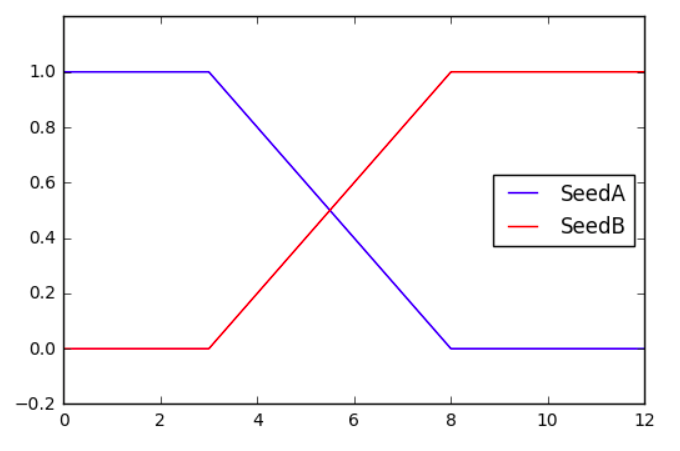
\includegraphics[scale = 0.4]{1_1.png}

\subsection{Implementation}

Below is our simple implementation of the random walker. We experimented with different seed positions and different values of $\gamma$. One can see that for small $\gamma$ the random walker doesn't properly respect the borders in the picture. For sufficiently large values of $\gamma$ the algorithm gives a satisfying result.

\begin{figure}
  \centering
  \includegraphics[width=\linewidth]{walker1}
  \includegraphics[width=\linewidth]{walker5}
\end{figure}

\begin{figure}
  \includegraphics[width=\linewidth]{walker10}
  \includegraphics[width=\linewidth]{walker100}
\end{figure}

\clearpage
\lstinputlisting[caption=random_walker.py,label=lst:rw]{random_walker.py}

\section{Random walker as Anisotropic Diffusion}
\[
\frac{\partial \phi}{\partial t} = D \frac{\partial^{2} \phi}{\partial x^{2}}
\]

When a large number of particles make randomwalk, diffusion equation describes the time developement of the particle density. I am going to show it.

Let's suppose that the particle at position x makes a random walk such that after time \(\Delta\)t, it moves to x+\(\Delta\)x with probability 1/2, x-\(\Delta\)x with probability 1/2.

Now, the following equation goes with regard to the particle density \(\phi\)

\[
\phi (x,t+\Delta t) = \frac{1}{2}\phi (x-\Delta x,t) + \frac{1}{2}\phi (x+\Delta x,t)
\]
Using Taylor expansion, it can be transformed as follows.

\[
\frac{\partial \phi}{\partial t} + O(\Delta t) = \frac{\Delta x^{2}}{\Delta t} \frac{\partial^{2} \phi}{\partial x^{2}} + O(\frac{\Delta x^{3}}{\Delta t})
\]

Take colloids in the water as a example of diffusion. They do brownian movement and their mean travel distance is proportional to the square root of time. For this reason, we can say that \(\frac{\Delta x^{2}}{\Delta t}\) is constant if we take \(\Delta\)x and \(\Delta\)t in proper range. Call constant D, by bringing \(\Delta\)x and \(\Delta\)t close to 0, we obtain a diffusion equation.

\end{document}
